%% LHS 1140b: the helium 10830 line from a solved wind (EXHALE) against the
%% isothermal Parker-wind retrieval of Cherubim et al. (2026) and against the
%% released measurement.  Records what was verified against the authors' own
%% code and data, where the two models part company, and what composition the
%% equivalent width implies.
%% Author: Kwang-Il Seon
\documentclass[english,a4paper]{my_memo}
\synctex=1
\usepackage{booktabs}
\usepackage{amsmath}
\usepackage{graphicx}
\usepackage{babel}
\emergencystretch=3em

\title{Reproducing the LHS\,1140\,b helium line with a solved wind:
       how far EXHALE gets, and what is missing}
\author{Kwang-Il Seon}
\date{Last updated: \docmoddate}

\begin{document}
\maketitle

\section{Goal, and the answer up front}

The objective is to reproduce the measured He\,\textsc{i} $10830$\,\AA{}
transit line of LHS\,1140\,b with EXHALE, which solves the wind rather than
imposing it, and to establish what --- if anything --- has to be added to
the physics for the model to match the observation.

\medskip
\noindent\textbf{Result.} EXHALE can be made to absorb the right
\emph{amount}: at $\mathrm{He/H} \simeq 0.55$ its equivalent width equals
the measured one to well within the observational error. It cannot
reproduce the \emph{line}. At that composition the profile is $3.4$ times
too deep and $3.4$ times too narrow, and no composition fixes this, because
composition changes how much helium absorbs, not how the absorption is
spread in velocity. Closing the gap needs $\simeq 22$\,km\,s$^{-1}$ FWHM of
velocity spread that the solved wind does not produce: its outflow reaches
$1.2$\,km\,s$^{-1}$ at $20\,R_p$ and its gas cools below $1000$\,K over the
line-forming region. The shortfall is in the energy and momentum budget,
not in the composition, and it is a published problem rather than a defect
of this setup (Sect.~\ref{sec:width}). The one mechanism that would supply
width without a free parameter---the adiabatic-cooling metastable bump of
Schulik \& Owen (2025)---is present in these solutions but sits at
$0.3$--$1.4$\,km\,s$^{-1}$, so it does not help (Sect.~\ref{sec:bump}).

Repeating the whole scan on the GJ\,699 proxy spectrum --- the second
stand-in for LHS\,1140's unobserved XUV, $5.1$ times brighter, which the
paper also uses --- separates the two questions (Sect.~\ref{sec:gj699}).
The escape rate rises sevenfold, to $4.0\times10^{8}$\,g\,s$^{-1}$, within
$0.04$\,dex of what the paper retrieves on that proxy, and the composition
the equivalent width implies moves from $\mathrm{He/H} = 0.55$ to $0.060$,
from helium-rich to below solar. The width gap is untouched: the added
broadening the measurement demands stays at $22$\,km\,s$^{-1}$. So the
composition inference is SED-limited, while the missing line width is not an
energy-input problem.

The paper's own p-winds fit does not reproduce the line either: it carries
roughly the right width, because its temperature is imposed at
$5000$--$6000$\,K where the line forms, but overshoots the blue component
threefold. Adding broadening does not rescue it: its absorbing power is
$24\%$ below the measurement, so no convolution can reach the observed
depth and width at once.

\medskip
\noindent Everything below uses inputs verified against the authors' own
released material (Zenodo 20723095): their p-winds driver script, their
Mega-MUSCLES v23 spectra, their reduced transmission spectrum and their
likelihood grid. Products live in \texttt{LHS1140b/}; the notebook
\texttt{LHS1140b/LHS1140b\_analysis.ipynb} regenerates every number and
figure here.

\section{Inputs, and how each was pinned}

\subsection{System}
Planet and star from Cadieux et al.\ (2024) as quoted by C26:
$R_p = 1.730 \pm 0.025\,R_\oplus$, $M_p = 5.60 \pm 0.19\,M_\oplus$,
$T_{\rm eq} = 226$\,K, $a = 0.0946$\,AU, $M_\star = 0.1844\,M_\odot$,
$R_\star = 0.2159\,R_\odot$. One trap: EXHALE converts $R_p$ with its own
internal constants (mean radii, $R_J = 6.9911\times10^{9}$\,cm,
$R_\oplus = 6.3725\times10^{8}$\,cm), so the input must be built with those
and not with IAU equatorial values --- a $2.2\%$ error in radius, $4.4\%$ in
transit depth, if taken from the wrong pair.

\subsection{Stellar spectrum}
\label{sec:sed}
The paper describes its normalization two ways that cannot both hold: the
Supplement's prose says the proxy SED is scaled so its integrated X-ray flux
matches that measured for LHS\,1140, while the quoted constants
($A_{1132} = 0.59$, $A_{699} = 0.056$) are the catalog X-ray flux
\emph{ratios}, a factor $1.8$ apart. The authors' script settles it:
\begin{verbatim}
Lx_ratio_1132 = 0.59
norm_constant_1132 = Lx_ratio_1132*(d_1140/(smax_1140*au2m))**2
\end{verbatim}
applied to the plain \texttt{const-res} v23 product. That combination also
reproduces the fiducial XUV flux the main text quotes, $0.033$\,W\,m$^{-2}$
(we measure $33.6$\,erg\,s$^{-1}$\,cm$^{-2}$ over $10$--$1300$\,\AA{}). All
results here use it. Note the proxy SED and the paper's own APEC fit
disagree in the X-ray band ($4.4$ against $2.9$\,erg\,s$^{-1}$\,cm$^{-2}$
at the orbit); that inconsistency is inherited from the paper's procedure,
not introduced here.

\subsection{Measurement}
The comparison target is the authors' released Fig.~3B spectrum (129
samples, vacuum, planetary rest frame, correlated-noise corrected), not a
reading of a figure. Fitting it with our own three-Gaussian extractor
(\texttt{he\_line\_metrics.py}, the same one applied to every model
spectrum here) reproduces the paper's MCMC to within its published
uncertainties:

\begin{center}
\begin{tabular}{lcc}
\toprule
 & this extractor & paper \\
\midrule
blended red depth & $1.254\%$ & $1.24^{+0.22}_{-0.23}\%$ \\
blue depth        & $0.198\%$ & $0.25^{+0.14}_{-0.12}\%$ \\
red/blue          & $6.35$    & $6.7^{+12.7}_{-3.1}$ \\
FWHM              & $0.841$\,\AA{} & $0.86^{+0.15}_{-0.27}$\,\AA{} \\
\bottomrule
\end{tabular}
\end{center}

\noindent so models and measurement can be compared through one instrument.

\section{Reproducing the paper's p-winds model}

Run at the authors' settings --- their SED normalization, $R_p = 0.154\,R_J$,
$b = 0.23$, \texttt{turbulence\_broadening=True}, five-phase transit
averaging, and their fitted line-of-sight bulk velocity
$v_{\rm wind} = 2.26$\,km\,s$^{-1}$ --- and at the MCMC medians
($\dot M = 2.03\times10^{8}$\,g\,s$^{-1}$, $T = 5160$\,K,
$\mathrm{H\!:\!He} = 1.01\times10^{-3}$), the vector their Fig.~4 legend
states for the plotted curve, our reproduction gives a red depth of
$1.376\%$ and FWHM $0.575$\,\AA{} against the $1.32\%$ and
$\sim 0.71$\,\AA{} read off their Fig.~4: a $3\%$ match in depth, but a
line about $20\%$ too narrow.

The width residual is not a consequence of which point in parameter space is
drawn. Running the same reproduction at the grid maximum-likelihood point
($1.83\times10^{8}$\,g\,s$^{-1}$, $5131.6$\,K, $8.338\times10^{-4}$) gives
red $1.366\%$ and FWHM $0.581$\,\AA{}, i.e.\ the two vectors differ by less
than $0.01$\,\AA{} in width. What produces the extra width in the published
curve has not been identified.

Two points are worth recording because both cost time to find.

First, the curves drawn over the spectrum in the paper's Fig.~3 are the
\emph{three-Gaussian empirical fits}, not p-winds; the physical model is
overlaid only in Fig.~4. Fig.~3's apparently perfect agreement is a fit to
the data, and says nothing about the model's line shape.

Second, the paper's plotted model is visibly broader than a plain p-winds
run, which we initially modelled as an undocumented instrumental kernel. It
is not: their script sets \texttt{turbulence\_broadening=True} and averages
over five transit phases. Both widen the line, and together they account for
the difference.

\section{Turbulent broadening: what the literature does}

Since that switch turned out to matter, all 43 papers under
\texttt{references/} were checked: every PDF converted to text, searched for
\texttt{turbulen}, \texttt{microturbulen} and \texttt{non-thermal
broadening}, and each hit read in context. Fifteen matched; most use
``turbulent'' for eddy diffusion $K_{zz}$ or for flow structure in 3D
simulations, not for line broadening. Section~\ref{sec:lit} tabulates the
ones that bear on broadening.

The convention, stated most explicitly by Yan et al.\ (2024), replaces the
thermal Doppler width by
\begin{equation}
  \Delta\nu_D = \frac{\nu_0}{c}\left(\frac{2kT}{m} + v_{\rm turb}^2\right)^{1/2},
  \qquad v_{\rm turb} = \sqrt{\frac{5kT}{3m}} = c_s ,
\end{equation}
the monatomic sound speed, as assumed by Salz et al.\ (2018), Lamp\'on et
al.\ (2020) and Czesla et al.\ (2022). The p-winds implementation uses
$\sqrt{5kT/6m}$ in a $\sigma$-convention, which is the same physics
expressed against a Doppler width that lacks the factor $2$; in EXHALE's
$b$-parameter convention the same term is $b \to \sqrt{11/6}\,v_{\rm th}$,
a factor $1.354$. That is what \texttt{EXHALE\_TRANSIT\_TURB=1} applies. It
is opt-in and off by default, because the field does not agree that it
belongs.

\subsection{Paper by paper}
\label{sec:lit}

\paragraph{Adopt it as an assumed value.}
\textbf{Salz et al.\ (2016)}, Eq.~(5): ``$b$ is the Doppler parameter,
$v_{\rm th}$ the thermal Doppler velocity, and for the microturbulence
$v_{\rm micro}$ we use the sound speed'', applied when synthesizing the
transit profile. (Their atmosphere solver separately carries a constant
$1$\,km\,s$^{-1}$ microturbulence at the lower boundary, a different
quantity, which they note ``has little impact on the overall atmospheric
structure''.) \textbf{Lamp\'on et al.\ (2020, 2021)} is the reference
implementation, with turbulent broadening as a free or assumed parameter of
1D isothermal Parker fits; \textbf{Czesla et al.\ (2022)} follows it.
\textbf{Cherubim et al.\ (2026)} inherits the choice through p-winds'
\texttt{turbulence\_broadening=True}, so the LHS\,1140\,b retrieval carries
it --- a fact stated nowhere in the paper text.

\paragraph{Test it, then leave it out.}
\textbf{Yan et al.\ (2024)} give the cleanest statement of the convention
and of the doubt. They record that ``these authors assumed that the
turbulence velocity $v_{\rm turb} = \sqrt{5kT/3m}$, which corresponds to the
speed of sound of a monatomic gas and, thus, to the transonic case with a
Mach number of 1'', then keep it out of their nominal models and test
$v_{\rm turb} = 0.5$, $1.0$ and $1.5\,c_s$ as a sensitivity. Their finding
for He\,10830 is that turbulence ``decreases the absorption depth slightly
at the line center, but doesn't significantly alter the absorption at the
line wings''. They argue Mach~1 is likely an overestimate, since in the
diffuse ISM turbulent velocity anti-correlates with temperature and the Mach
number is below unity at a few thousand K, and conclude ``the turbulence
effect is likely less significant than the one explored in this paper''.
\textbf{Yan et al.\ (2019)} computes the Doppler width explicitly
``assuming no turbulence''.

\paragraph{Argue against it.}
\textbf{Murray-Clay et al.\ (2009)}, on Garc\'ia Mu\~noz's (2007) proposal
to broaden Ly$\alpha$ by wind turbulence: ``to generate the large velocities
observed, the energy in such turbulence would need to exceed the thermal and
bulk kinetic energies in the mean flow by a factor of $\sim 100$. Such
energy requirements seem insurmountable.'' \textbf{Koskinen et al.\ (2013b)}
find that ``non-thermal broadening such as that proposed by Ben-Jaffel and
Hosseini (2010) does not appear to be necessary to explain the current
observations'', while allowing that stellar-wind interaction may produce
broadening turbulence. \textbf{Schulik \& Owen (2025)} offer a physical
alternative --- adiabatic cooling produces a metastable-helium population
bump at high velocity, widening the line with no free parameter --- and are
pointed about the alternative: the isothermal model ``can only explain the
broadness of the data under physically inconsistent assumptions, i.e.\ those
of even larger mass-loss rates, not supported by the energy input into this
planet, and an empirical free parameter, turbulent broadening (Lamp\'on et
al.\ 2021)''. They add that $T = 10^{4}$\,K already maximizes what thermal
broadening alone can give.

\paragraph{Need it even so.}
\textbf{Taylor et al.\ (2026)} is the closest analogue to the present work:
a self-consistent model (energy balance, multispecies diffusion, non-LTE
H($n=2$)) that reproduces the HD\,189733\,b line core but not its width.
They write that ``several prior analyses have matched the HD\,189733\,b width
by introducing ad hoc (micro)turbulent or Gaussian broadening terms; here, we
show that this step remains necessary even in our self-consistent
framework'', and quantify it as $\sim 12$\,km\,s$^{-1}$ of additional
non-thermal broadening. They speculate --- explicitly calling it speculative
--- that it is plasma turbulence from ions trapped on low-latitude planetary
field lines, strengthening with stellar activity.
\textbf{Rumenskikh et al.\ (2022)}, as reported there, instead imposed
reduced hydrogen line cooling and prescribed zonal jets of
$10$--$20$\,km\,s$^{-1}$ in a 3D multifluid model.

\paragraph{Matches that are not about broadening.}
Recorded so the sweep need not be repeated: Wogan (2025), Lavvas (2014,
2019), Robeling (2026) and the second half of Koskinen et al.\ (2013b) use
``turbulent'' for eddy diffusion $K_{zz}$; \texttt{2607.18193v1} for
flow--flow interaction in a 3D stellar-wind simulation; Jensen (2012) for
photospheric turbulence driving stellar activity; Taylor et al.\ (2025) for
gravity-wave breaking. \texttt{Vidal\_2003\_Nature.pdf} matches only on its
first page, which carries the tail of the preceding \textit{Nature} letter
(on Crab pulsar radio emission); Vidal-Madjar et al.\ themselves do not
discuss turbulence.

\paragraph{Where that leaves this comparison.}
There is no settled treatment. Turbulence at $v_{\rm turb} = c_s$ is a
common convention in 1D isothermal Parker-wind fits --- and hence in the
paper being reproduced --- while self-consistent and 3D models either need a
larger ad hoc term, reach the width by other physics, or argue the term is
unjustified. Enabling it here is therefore right for a like-for-like
comparison and wrong as a default, which is how it is implemented.

\section{Searching for a match: the composition scan}

Composition is the one free parameter of the problem once the star, the
planet and the spectrum are fixed, so it is where a match has to be sought
first. Eleven compositions were solved, from solar ($\mathrm{He/H} = 0.083$)
to $\mathrm{He/H} = 10^{4}$, each a JFNK steady state
($\|R\| < 10^{-3}$, \texttt{info}~$=0$; one case, $\mathrm{He/H} = 100$,
stagnates at $1.18\times10^{-3}$ and is recorded as such). Nothing is
imposed: mass, momentum and energy are solved with photoionization heating
and radiative cooling, so $\dot M$ and $T(r)$ are outputs.

\begin{center}
\begin{tabular}{rccccc}
\toprule
$\mathrm{He/H}$ & $\log_{10}\dot M$ & red & red (turb) & FWHM & EW \\
 & [g\,s$^{-1}$] & [\%] & [\%] & [\AA] & [\%\,\AA] \\
\midrule
$0.083$ & $7.77$ & $1.21$  & $1.08$  & $0.218$ & $0.279$ \\
$0.25$  & $7.75$ & $2.65$  & $2.32$  & $0.230$ & $0.645$ \\
$0.50$  & $7.76$ & $4.05$  & $3.50$  & $0.242$ & $1.040$ \\
$0.55$  & $7.76$ & $4.29$  & $3.69$  & $0.244$ & $1.109$ \\
$0.70$  & $7.78$ & $4.97$  & $4.26$  & $0.248$ & $1.311$ \\
$1$     & $7.80$ & $5.88$  & $5.01$  & $0.255$ & $1.598$ \\
$10$    & $7.76$ & $75.97$ & $73.11$ & $0.267$ & $21.53$ \\
$10^{3}$& $7.74$ & $73.39$ & $70.06$ & $0.269$ & $20.97$ \\
$10^{4}$& $7.73$ & $72.78$ & $69.44$ & $0.268$ & $20.78$ \\
\midrule
observed & --- & $1.254$ & --- & $0.841$ & $1.108 \pm 0.030$ \\
\bottomrule
\end{tabular}
\end{center}

The escape rate is nearly composition-independent,
$\dot M \simeq 6\times10^{7}$\,g\,s$^{-1}$, about a third of the
$2.03\times10^{8}$ the retrieval imposes.

\begin{figure}[htbp]\centering
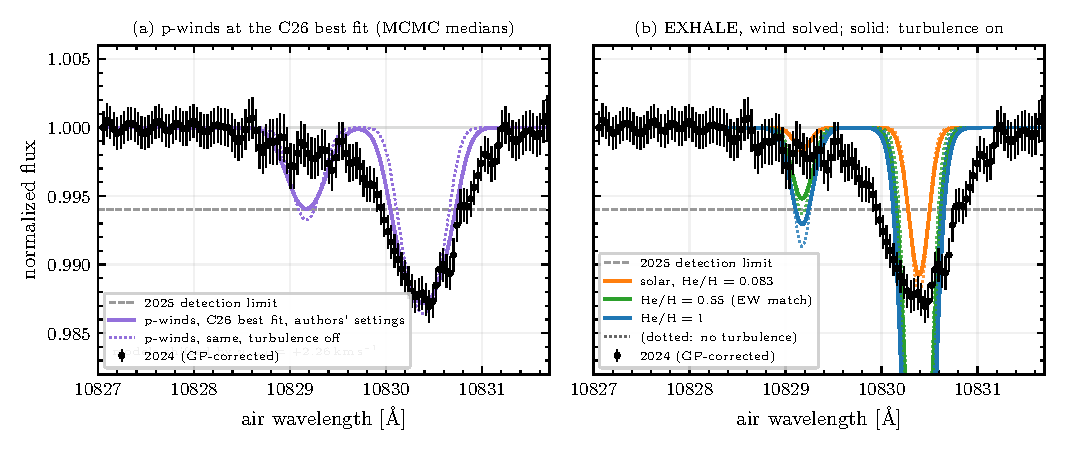
\includegraphics[width=\textwidth]{figures/lhs1140b_fig4style.pdf}
\caption{The measurement (black) with, left, the paper's own p-winds model
at its best fit --- the MCMC medians its Fig.~4 legend states --- computed
with the authors' released settings (solid;
dotted is the same run with turbulence off), and right, EXHALE at three
compositions. Solid EXHALE curves carry the same turbulence
term p-winds uses; dotted are without it. Neither code applies a
line-of-sight bulk velocity, so both sets of model curves are shifted by the
$v_{\rm wind} = +2.26$\,km\,s$^{-1}$ that C26 fit; the shift is rigid and
leaves equivalent widths unchanged. Drawn in the presentation of the paper's
Fig.~4.}
\label{fig:fig4}
\end{figure}

\section{Why the two models disagree}

At the same composition the two models are not small perturbations of each
other. The \emph{total} metastable column is comparable --- at
$\mathrm{H\!:\!He} = 10^{-3}$ EXHALE's is about half of p-winds' --- but its
distribution is not, and transit depth is absorbing \emph{area}:

\begin{center}
\begin{tabular}{lcc}
\toprule
 & p-winds & EXHALE \\
\midrule
$50\%$ of the $2\,^3S$ column inside & $1.33\,R_p$ & $5.7\,R_p$ \\
$90\%$ inside                        & $1.59\,R_p$ & $10.2\,R_p$ \\
\bottomrule
\end{tabular}
\end{center}

The star is $13.6\,R_p$ across, so metastable helium spread to $10\,R_p$
covers most of the disk while a column confined to $1.6\,R_p$ can darken
only a narrow ring. The distribution difference is the wind structure ---
the one thing p-winds imposes and EXHALE solves. At $r = 10\,R_p$, same
composition and spectrum: p-winds is isothermal at $6100$\,K by
construction, EXHALE's energy balance gives $1392$\,K; p-winds flows at
$4.3$\,km\,s$^{-1}$, EXHALE at $0.53$; and the cold, slow, denser gas keeps
helium neutral and the metastable level populated far out,
$n(2\,^3S) = 40$\,cm$^{-3}$ against $2\times10^{-4}$
(Fig.~\ref{fig:structure}).

\begin{figure}[htbp]\centering
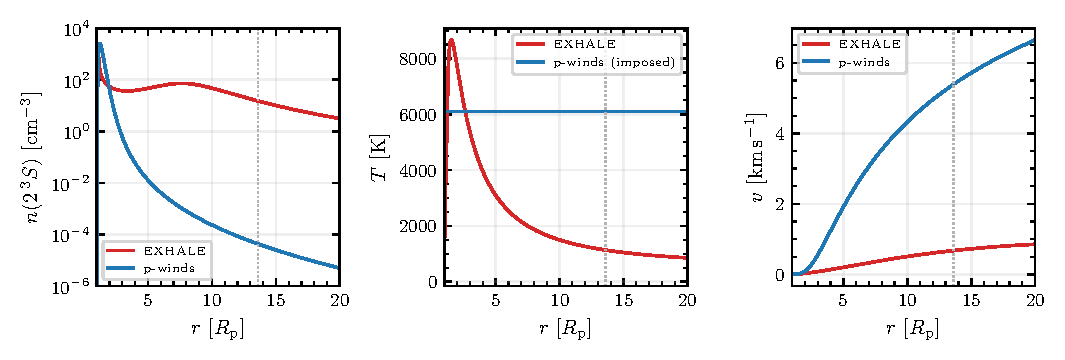
\includegraphics[width=\textwidth]{figures/lhs1140b_structure.pdf}
\caption{Same composition ($\mathrm{H\!:\!He} = 10^{-3}$), same spectrum,
two wind structures. Dotted vertical line: the stellar radius, $13.6\,R_p$.}
\label{fig:structure}
\end{figure}

\section{What can be matched: the equivalent width}

Depth and width trade against each other under any broadening, but the
equivalent width does not: it is invariant under the instrument profile, the
turbulence term and the phase averaging. It is therefore the quantity on
which a self-consistent model can be matched without first settling the
broadening question.

Over the blended red pair (vacuum $10832.6$--$10834.2$\,\AA), the released
spectrum gives $EW = 1.108 \pm 0.030$\,\%\,\AA. EXHALE crosses it at

\begin{equation}
  \mathrm{He/H} \simeq 0.55 \quad (0.53\text{--}0.57 \text{ on the } EW\
  1\sigma), \qquad \mathrm{H\!:\!He} \simeq 1.8 ,
\end{equation}

that is $6.6\times$ solar, a helium mass fraction of $0.69$. Enabling
turbulence moves this to $0.541$, a $1.6\%$ shift --- a direct demonstration
that the estimate does not depend on the broadening treatment. The value
sits three orders of magnitude away from the paper's
$\mathrm{H\!:\!He} \lesssim 10^{-3}$, and the reason is the structural
difference of the previous section: a wind that spreads metastable helium
over most of the stellar disk needs far less helium to absorb as much.

\begin{figure}[htbp]\centering
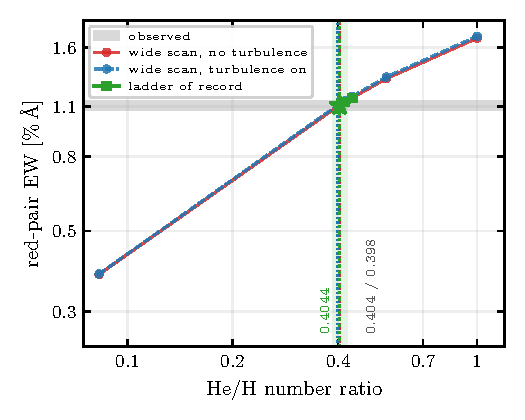
\includegraphics[width=0.55\textwidth]{figures/lhs1140b_ew_vs_heh.pdf}
\caption{Red-pair equivalent width against composition, with and without the
turbulence term, against the measured band. The crossing is insensitive to
the broadening treatment.}
\label{fig:ew}
\end{figure}

\section{What cannot be matched: the profile}
\label{sec:width}

Matching the equivalent width is not matching the line. At
$\mathrm{He/H} = 0.55$ the profile is $3.4$ times too deep ($4.29\%$ against
$1.254\%$) and $3.4$ times too narrow ($0.244$ against $0.841$\,\AA). The
equivalent width states how much absorbing power the model has; the profile
states how that power is spread in velocity, and composition does not act on
the second. Every solved composition gives $0.22$--$0.27$\,\AA{}, rising
only to $0.24$--$0.31$\,\AA{} with the turbulence term.

\subsection{How much is missing, in velocity}

The measured FWHM is $0.841$\,\AA, that is $23.3$\,km\,s$^{-1}$ at
$10833$\,\AA. Three ways to supply it, and what each would require:

\begin{itemize}
\item \emph{Thermal alone.} A Doppler width of $23.3$\,km\,s$^{-1}$ FWHM in
      helium needs $T = 4.7\times10^{4}$\,K. Helium is fully ionized far
      below that, so there would be no metastable population left to
      absorb. This is excluded.
\item \emph{Bulk outflow.} A line-of-sight velocity spread of order
      $\pm 12$\,km\,s$^{-1}$ across the line-forming region would do it.
      The EW-matched EXHALE solution reaches $1.2$\,km\,s$^{-1}$ at
      $20\,R_p$; the paper's p-winds model, with its imposed temperature,
      reaches $4$--$7$. Both are an order of magnitude short.
\item \emph{Non-thermal (turbulent) broadening.} Added in quadrature to
      what EXHALE already has, closing the gap takes
      $22.3$\,km\,s$^{-1}$ FWHM --- $9.5$\,km\,s$^{-1}$ of turbulent
      velocity ($\sigma$), against the $2.9$\,km\,s$^{-1}$ that the
      sound-speed convention of Sect.~\ref{sec:lit} supplies for
      helium at $5000$\,K. This is the one of the three that can be measured
      directly, and Sect.~\ref{sec:broadening} measures it.
\end{itemize}

\noindent So the model is not short by a detail. It is short by an amount
of velocity comparable to the escape speed, and no choice of composition
supplies it.

\subsection{The broadening the data demand, measured}
\label{sec:broadening}

The three routes above can be replaced by one measurement. Take the
EW-matched EXHALE profile as solved, convolve it with a Gaussian of FWHM
$f$ in velocity, and ask which $f$ reproduces the measured line. The
convolution is applied to the excess absorption
$(\max T - T)/\max T$ built from the instrument-convolved column of
\texttt{tpm\_He10830.txt}; depth, width and the red/blue ratio are then read
off with the same three-Gaussian extractor applied to the data, and the
equivalent width by the same integral over the vacuum window
$10832.60$--$10834.20$\,\AA. So $f$ is the only quantity varied, and every
number in Table~\ref{tab:broadening} is measured the way the corresponding
observed number was.

\begin{table}[htbp]\centering
\caption{The EW-matched EXHALE profile ($\mathrm{He/H} = 0.55$, no
turbulence term) convolved with an added Gaussian of FWHM $f$. Observed
values on the last row: red and blue depths from the C26 MCMC posterior,
width and equivalent width measured here on their spectrum.}
\label{tab:broadening}
\begin{tabular}{lrrrrr}
\toprule
$f$ [km\,s$^{-1}$] & red [\%] & blue [\%] & red/blue & FWHM [\AA] &
EW [\%\,\AA] \\
\midrule
$0$   & $4.285$ & $0.624$ & $6.86$ & $0.244$ & $1.109$ \\
$10$  & $2.393$ & $0.321$ & $7.45$ & $0.435$ & $1.109$ \\
$15$  & $1.754$ & $0.232$ & $7.56$ & $0.593$ & $1.106$ \\
$20$  & $1.366$ & $0.180$ & $7.61$ & $0.762$ & $1.090$ \\
$\mathbf{22.3}$ & $\mathbf{1.237}$ & $\mathbf{0.162}$ & $\mathbf{7.62}$ &
$\mathbf{0.841}$ & $\mathbf{1.076}$ \\
$25$  & $1.114$ & $0.146$ & $7.63$ & $0.935$ & $1.056$ \\
\midrule
observed & $1.24^{+0.22}_{-0.23}$ & $0.25^{+0.14}_{-0.12}$ &
$6.7^{+12.7}_{-3.1}$ & $0.841$ & $1.108 \pm 0.030$ \\
\bottomrule
\end{tabular}
\end{table}

The width is reached at $f = 22.3$\,km\,s$^{-1}$ FWHM, that is
$\sigma = 9.5$\,km\,s$^{-1}$. At that one value the depth is $1.237\%$
against the measured $1.24^{+0.22}_{-0.23}$, the blue component $0.162\%$
against $0.25^{+0.14}_{-0.12}$, and the ratio $7.62$ against
$6.7^{+12.7}_{-3.1}$: depth, blue depth and ratio all land inside the
observed $1\sigma$ interval at the value fixed by the width alone. Nothing
was tuned to them. Figure~\ref{fig:broadened} shows the profile and the two
crossings.

The number does not depend on which solution is broadened. The same
crossing is at $21.9$\,km\,s$^{-1}$ for the $\mathrm{He/H} = 0.55$ run with
the turbulence term already on, and at $22.5$\,km\,s$^{-1}$ for solar
composition --- although the solar run is a quarter of the observed
absorption ($0.311\%$ red, EW $0.270$) and so matches the shape while
missing the amount. The required broadening is therefore set by the
velocity field, not by composition or by the broadening treatment already
in place: the direct measurement of what Sect.~\ref{sec:width} inferred.
The equivalent width falls by $3\%$ between $f = 0$ and $f = 22.3$ because
the Gaussian wings carry absorption out of the red-pair integration
window, not because absorbing power is lost.

This is descriptive, not explanatory. It states that one free parameter,
applied to a solved profile, reproduces the measured line; it does not say
what produces $22.3$\,km\,s$^{-1}$. The candidates are the ones listed
below, and the measurement sharpens them by fixing the number each has to
deliver.

One conversion narrows the list before it is read. If the missing
$22.3$\,km\,s$^{-1}$ is called turbulence, it has to be turbulence in gas
whose sound speed the solution itself fixes. Evaluating
$c_s = (\gamma kT/\mu m_H)^{1/2}$ with $\gamma = 5/3$ on the
$\mathrm{He/H} = 0.55$ output, taking $\mu$ from the solved
H\,\textsc{i}/H\,\textsc{ii}/He\,\textsc{i}/He\,\textsc{ii}/He\,\textsc{iii}
and electron densities, gives $c_s = 5.5$\,km\,s$^{-1}$ at $2\,R_p$
($T = 4311$\,K, $\mu = 1.94$), $3.8$ at the metastable peak $5.4\,R_p$
($1609$\,K, $1.57$) and $3.0$ at $10\,R_p$ ($845$\,K, $1.32$); weighted over
the line-forming region by $n(2\,^3S)\,r$, $T = 2022$\,K, $\mu = 1.59$ and
$c_s = 3.9$\,km\,s$^{-1}$. Note this is the bulk-gas sound speed, the
quantity a Mach number is defined against, and not the helium thermal speed
that enters the line profile.

Against that, the kernel is supersonic on any convention. Read as a
line-of-sight velocity dispersion, $\sigma = 9.5$\,km\,s$^{-1}$ is
$\mathcal{M} = 2.4$. Read in the $b$-parameter convention of Lamp\'on et
al.\ and p-winds, where $v_{\rm turb}$ is the quantity added to
$b^2 = 2kT/m + v_{\rm turb}^2$, it is $v_{\rm turb} = \sqrt{2}\,\sigma =
13.4$\,km\,s$^{-1}$, $\mathcal{M} = 3.4$; as an isotropic three-dimensional
turbulent speed, $\sqrt{3}\,\sigma = 16.4$\,km\,s$^{-1}$,
$\mathcal{M} = 4.2$. The $v_{\rm turb} = c_s$ convention of
Sect.~\ref{sec:lit} supplies only $3$--$4$\,km\,s$^{-1}$ in this gas, about
a third of what the data demand. That is the opposite corner of the
literature reviewed there: Yan et al.\ (2024) argue $\mathcal{M} = 1$ is
already an overestimate at a few thousand K, and Murray-Clay et al.\ (2009)
call the energy requirement of supersonic turbulence ``insurmountable''.
Supplying the shortfall under the name of turbulence therefore looks
physically hard to sustain, and the measurement points to the candidates of
the next section --- an ordered velocity field, three-dimensional flow, or
heating the 1D energy equation does not carry --- rather than to a missing
thermal width.

\begin{figure}[htbp]\centering
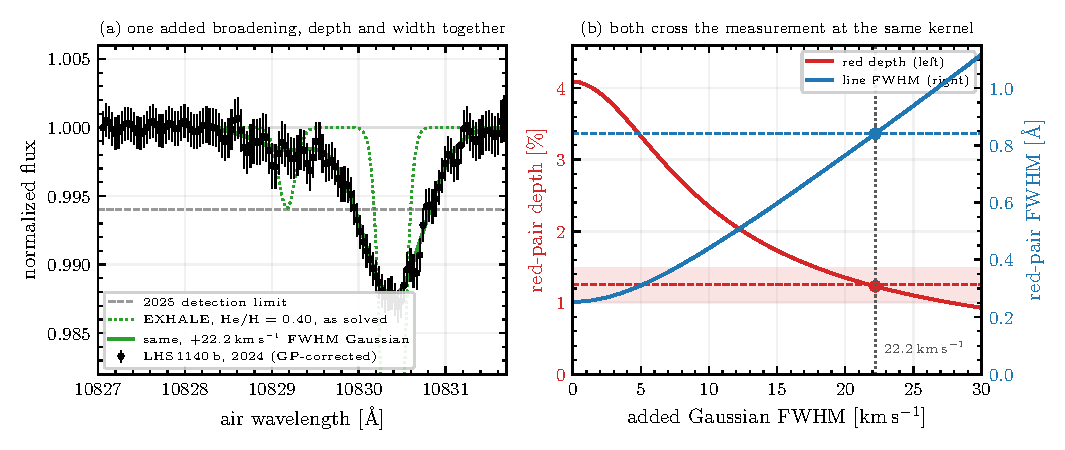
\includegraphics[width=\textwidth]{figures/lhs1140b_broadened.pdf}
\caption{Left: the EW-matched EXHALE profile as solved (dotted, its core
running below the plotted range) and convolved with a $22.3$\,km\,s$^{-1}$
FWHM Gaussian (solid), against the measurement. Both are shifted by the
same $v_{\rm wind} = +2.26$\,km\,s$^{-1}$ used in the earlier figures.
Right: red-pair depth (red, left axis) and red-pair FWHM (blue, right axis)
as the added kernel is scanned. Dashed lines are the observed values, the
shaded band the C26 $1\sigma$ interval on the depth; the dotted vertical
marks where the width is matched. Both curves meet the measurement at the
same kernel.}
\label{fig:broadened}
\end{figure}

\subsection{Broadening cannot repair a deficit in equivalent width}
\label{sec:pwbroad}

The same scan was applied to the p-winds curves, in their own vacuum frame
and with the same three-Gaussian extractor and the same integration window
(Table~\ref{tab:pwbroad}). The convolution conserves absorbing power: it
redistributes the excess in velocity and leaves the equivalent width
unchanged, apart from the few percent that the wings carry out of the
integration window. Whether one kernel can reproduce depth and width
together is therefore decided before the scan starts, by the equivalent
width the curve already has at $f = 0$.

\begin{table}[htbp]\centering
\caption{The same added-Gaussian scan applied to the p-winds curves, with
the EXHALE row of Table~\ref{tab:broadening} repeated for comparison. The
kernel is the one that reproduces the measured width, $0.841$\,\AA; the
depths and the ratio are read at that kernel. Equivalent widths are for the
unbroadened curve, over the vacuum window
$10832.60$--$10834.20$\,\AA.}
\label{tab:pwbroad}
\begin{tabular}{lrrrrr}
\toprule
curve & EW$(f{=}0)$ [\%\,\AA] & $f$ [km\,s$^{-1}$] & red [\%] & blue [\%] &
red/blue \\
\midrule
p-winds best fit, turbulence on  & $0.837$ & $17.8$ & $0.926$ & $0.339$ &
$2.73$ \\
p-winds best fit, turbulence off & $0.701$ & $20.1$ & $0.777$ & $0.301$ &
$2.58$ \\
p-winds depth-matched, $6100$\,K & $0.480$ & $20.2$ & $0.535$ & $0.140$ &
$3.82$ \\
EXHALE, $\mathrm{He/H} = 0.55$   & $1.109$ & $22.3$ & $1.237$ & $0.162$ &
$7.62$ \\
\midrule
observed & $1.108 \pm 0.030$ & --- & $1.24^{+0.22}_{-0.23}$ &
$0.25^{+0.14}_{-0.12}$ & $6.7^{+12.7}_{-3.1}$ \\
\bottomrule
\end{tabular}
\end{table}

The p-winds best fit carries $0.837$\,\%\,\AA{} against the measured
$1.108 \pm 0.030$, $24\%$ short. At the kernel that reproduces the width,
$f = 17.8$\,km\,s$^{-1}$, the red depth is $0.926\%$ against
$1.24^{+0.22}_{-0.23}$, about $1.4\sigma$ low. What the broadening does is
move the disagreement rather than remove it: unbroadened, the curve is too
deep in the blue component ($0.534\%$ against $0.25^{+0.14}_{-0.12}$, some
$2\sigma$ high) and too narrow; broadened to the measured width, the blue
component falls to $0.339\%$, inside $1\sigma$, and the red component drops
below the measurement. The blue side is genuinely improved; the red side is
not, and the total is fixed.

The intensity ratio barely moves, $2.57$ at $f = 0$ against $2.73$ at the
matched kernel. It is the amplitude ratio of a saturated pair, set by how
the two components share the optical depth, and a common convolution acts
on both alike. It stays well below the measured $6.7^{+12.7}_{-3.1}$,
though the observed interval is wide enough that this alone is not a
discriminator.

Matching the depth as well would require $24\%$ more absorbing power, and
that is not something a kernel supplies: it is a change in $\dot M$,
temperature or composition. Fitting the broadening as a free parameter
alongside those --- which is what the measurement asks for --- would
presumably shift the C26 parameter estimates, since the composition is
constrained through the same absorbing power that would have to rise.

The asymmetry with EXHALE should not be read as one code outperforming the
other. The EXHALE curve entered the scan with its equivalent width already
set to the observed value by the choice of $\mathrm{He/H} = 0.55$
(Sect.~\ref{sec:broadening}), so only the shape remained free, and one
kernel settled it. The p-winds curve entered at the composition C26 report,
whose equivalent width falls short, so no kernel could settle both. The two
scans test the same physical statement --- broadening redistributes, it
does not create --- from two different starting points.

\begin{figure}[htbp]\centering
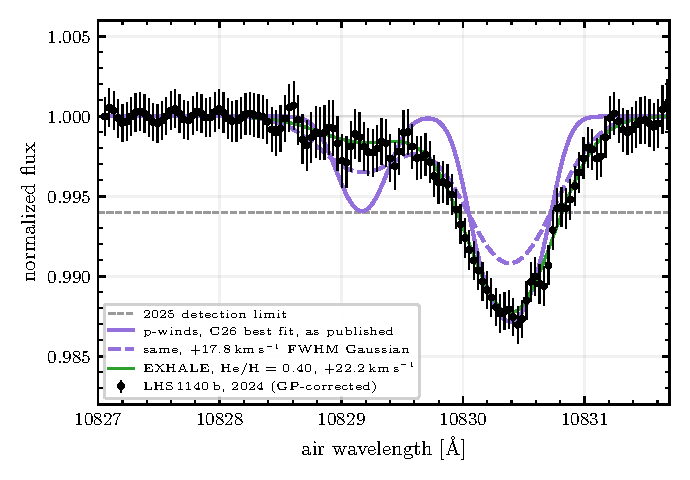
\includegraphics[width=0.60\textwidth]{figures/lhs1140b_pwinds_broadened.pdf}
\caption{The C26 p-winds best fit as published (solid purple) and convolved
with the $17.8$\,km\,s$^{-1}$ FWHM Gaussian that reproduces the measured
width (dashed purple), against the measurement; the EXHALE
$\mathrm{He/H} = 0.55$ curve at its own matched kernel
($22.3$\,km\,s$^{-1}$, thin green) is repeated from
Fig.~\ref{fig:broadened}. Broadened to the observed width, the p-winds
curve passes above the red core: the width is matched and the depth is not.
All curves are shifted by the same $v_{\rm wind} = +2.26$\,km\,s$^{-1}$.}
\label{fig:pwbroad}
\end{figure}

\subsection{The adiabatic-cooling population bump, looked for}
\label{sec:bump}

Schulik \& Owen (2025) propose that the missing width is already contained
in the metastable population itself. Writing the steady state of their
Eq.~(1) as
%
\begin{equation}
n_{2^3S}(T_e) = \frac{\alpha(T_e)}{q(T_e) + t_{\rm ion}/n_e}\,n_{\rm He^+},
\end{equation}
%
they note that as adiabatic expansion drops the temperature ``from $\simeq
10^4$\,K to $\simeq 10^3$\,K'', ``a change in slope in the population occurs
as the dominant triplet loss rate $q(T_e)$ drops significantly at lower
temperatures''---the metastable fraction climbs above the curve computed
with the rates frozen at the peak temperature. The rise is ``quenched'' where
the advection timescale overtakes the excitation to $2^1S$, after which
$\dot m_{2^3S} = 4\pi r^2 v\,n_{2^3S}\,m_{\rm He}$ falls through
ionization and the $2^3S \rightarrow 1^1S$ decay. They credit Yan et al.\
(2022) and Biassoni et al.\ (2024) with first identifying the effect, and
their conclusion states the condition it must satisfy to be observable:
``The helium triplet population bump must be situated at high velocities to
help explain anomalous line widths.''

EXHALE carries the temperature dependence the mechanism needs, and carries it
in exactly the balance above. The metastable row
(\texttt{tr\_triplet\_row}, \texttt{ion\_residual\_core.f90}:72) is
%
\begin{equation}
\begin{split}
n_e\bigl(n_{\rm He^+}\alpha_{2^3S} + n_{\rm He\,I(1^1S)}\,q_{13}\bigr)
 = \; & n_{2^3S}\bigl[\Gamma_{2^3S} + A_{31} + n_{\rm H\,I}Q_{31} \\
      & + n_e(q_{31a}+q_{31b}+b_{2^3S})\bigr],
\end{split}
\end{equation}
%
with every coefficient a function of $T$: $\alpha_{2^3S} = 2.10\times
10^{-13}(T/10^4)^{-0.778}$ (\texttt{Cool\_coeff.f90}:970), the collisional
losses $q_{31a}$ ($2^3S \rightarrow 2^1S$, $0.80$\,eV) and $q_{31b}$
($2^3S \rightarrow 2^1P$, $1.40$\,eV) as Bray (2000) collision strengths
folded with $\exp(-\Delta E/kT)$ (\texttt{Cool\_coeff.f90}:905 and 928), the
Penning term $Q_{31}$ as the Taylor et al.\ (2025) two-branch fit
(\texttt{Cool\_coeff.f90}:988), collisional ionization of the metastable
(\texttt{Cool\_coeff.f90}:1030), and the radiative decay $A_{31} =
1.272\times10^{-4}$\,s$^{-1}$ (\texttt{util\_ion\_eq.f90}:1192). Between
$5000$ and $1000$\,K the loss $q_{31a}+q_{31b}$ falls by a factor $1.3\times
10^{3}$ while $\alpha_{2^3S}$ rises by a factor $3.5$, so the
ingredients of the bump are present and are not an imposed
parameterization.

\texttt{LHS1140b/bump\_analysis.py} measures the result. It reconstructs the
balance above in Python from the solved profiles---reproducing the solved
$n_{2^3S}$ to a relative $3\times10^{-16}$, which confirms the rate
transcription and lets the one unresolved term, the $2^3S$ photoionization
rate $\Gamma_{2^3S}$, be recovered from the solution itself---and then
recomputes the reference curve with $\alpha$, $q_{13}$, $q_{31a}$, $q_{31b}$
and $Q_{31}$ frozen at the peak temperature.

\begin{table}[htbp]\centering
\caption{The metastable bump in the converged solutions. Columns 2--4
locate the $n_{2^3S}$ maximum in the equilibrium profile and give the
temperature and outflow speed there; the last three characterize the
absorber-weighted ($w = n_{2^3S}r^2\,dr$) distribution of $|v_r|$ over the
advection-corrected $2^3S$ column that the transit tool integrates. The
He/H\,$=1000$ solutions have no outward density maximum---their $n_{2^3S}$
peaks at the base---and are marked $\dagger$.}
\label{tab:bump}
\begin{tabular}{lrrrrrr}
\toprule
case & $r_{\rm peak}$ & $T$ & $v$ & med.\ $|v_r|$ & $>2$ & $>5$ \\
     & [$R_p$] & [K] & [km\,s$^{-1}$] & [km\,s$^{-1}$] & [\%] & [\%] \\
\midrule
\multicolumn{7}{l}{\emph{GJ\,1132 proxy SED}}\\
He/H\,$=0.55$   & $5.42$ & $1608$ & $0.27$ & $0.38$ & $0.0$ & $0.0$ \\
solar He/H      & $3.02$ & $1876$ & $0.07$ & $0.41$ & $0.0$ & $0.0$ \\
He/H\,$=1000$   & $1.05^\dagger$ & $2550$ & $0.00$ & $0.52$ & $0.0$ & $0.0$ \\
\midrule
\multicolumn{7}{l}{\emph{GJ\,699 proxy SED}}\\
He/H\,$=0.06$   & $5.42$ & $1015$ & $1.40$ & $2.53$ & $64.9$ & $0.0$ \\
solar He/H      & $5.50$ & $1047$ & $1.41$ & $2.51$ & $64.3$ & $0.0$ \\
He/H\,$=1000$   & $1.05^\dagger$ & $2529$ & $0.00$ & $1.40$ & $11.3$ & $0.0$ \\
\bottomrule
\end{tabular}
\end{table}

The bump is there. In every case the metastable fraction $f_3 =
n_{2^3S}/n_{\rm He}$ rises monotonically outward across the whole cooling
leg, from the temperature maximum to a maximum of $f_3$ at
$8.3$--$16.2\,R_p$---a rise of $1.4$--$4.2\times10^{3}$ in the equilibrium
profiles and $38$--$1.1\times10^{3}$ in the advection-corrected ones---and the rise is
attributable to the temperature dependence in the way Schulik \& Owen
describe: against the same balance with the rates frozen at the peak
temperature, the solved population stands a factor $1.6$--$31$ high at the
density maximum and up to $8.8$--$156$ high further out. On the GJ\,1132
proxy at the equivalent-width-matched composition the maximum sits at
$5.42\,R_p$ where $T = 1608$\,K, against $T_{\rm max} = 5043$\,K at
$1.45\,R_p$: the temperature has fallen to $0.32$ of its peak, which is the
regime the mechanism asks for. The quench is visible too---in the
advection-corrected profiles the density maximum has moved inward to
$1.05$--$1.64\,R_p$ and $n_{2^3S}$ then falls monotonically, so the outflow
appears to be sweeping the metastable out at least as fast as recombination
resupplies it, and $\dot m_{2^3S}$ drops by up to $41\%$ past the peak.

The velocity condition, however, is not met, and not narrowly. At the bump
the outflow is moving at $0.27$\,km\,s$^{-1}$ on the GJ\,1132 proxy and
$1.4$\,km\,s$^{-1}$ on the GJ\,699 proxy. Weighting by absorbers over the
whole $2^3S$ column, the median $|v_r|$ is $0.4$--$0.5$\,km\,s$^{-1}$ and
$2.5$\,km\,s$^{-1}$ on the two spectra, and the largest $|v_r|$ anywhere in
the column is $1.6$ and $3.9$\,km\,s$^{-1}$. No part of the column on
either spectrum reaches $5$\,km\,s$^{-1}$, against the $\sigma
= 9.5$\,km\,s$^{-1}$ of extra broadening the measurement demands
(Sect.~\ref{sec:broadening}). Radial velocity is the generous choice here:
the line-of-sight projection of a radial field over the transit chord is
smaller still. Figure~\ref{fig:bump} shows the three statements together.

So the bump exists in these solutions and contributes nothing measurable to
the width. That is consistent with what Schulik \& Owen themselves report
for the coolest hosts: for their M2 case they find that ``the transit
signal probes the same velocity region for both treatments of
thermodynamics, making the line insensitive to velocity'', and they conclude
that K stars, not M stars, are the favorable testbeds---G-type hosts
suppress the bump by photoionizing the triplet, and M-type hosts have weaker
tidal fields and so rarely drive fast enough outflows. LHS\,1140 is an M4.5
dwarf, cooler than the M2 they model, and its planet is a temperate
super-Earth rather than a hot giant. The mechanism appears to be present and
correctly captured; the host is the wrong one for it to help.

\begin{figure*}[htb]\centering
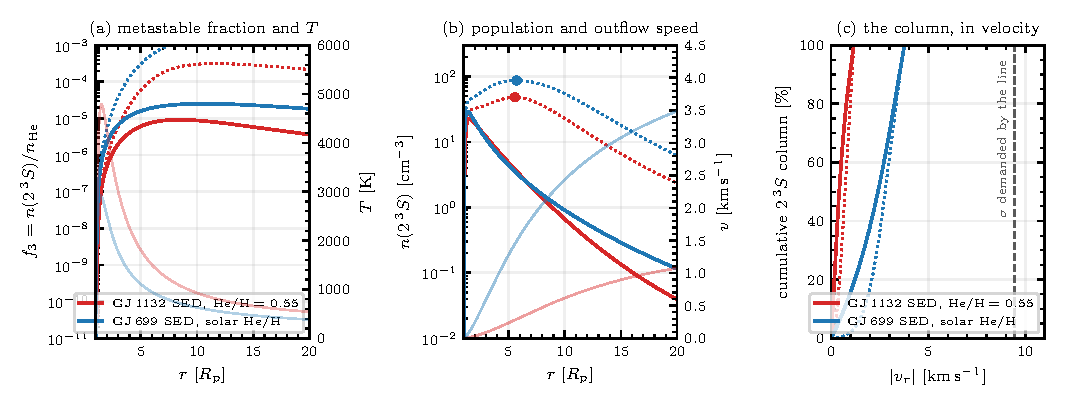
\includegraphics[width=0.98\textwidth]{figures/lhs1140b_bump.pdf}
\caption{The adiabatic-cooling metastable bump in the EXHALE solutions
(solid: advection-corrected, the profiles the transit integral uses;
dotted: local equilibrium; faint curves on the right-hand axes). (a) The
metastable fraction rises outward over the whole region where $T$ falls,
which is the bump in the sense of Schulik \& Owen (2025). (b) The
equilibrium $n_{2^3S}$ peaks at $5.4$--$5.5\,R_p$ (markers); advection moves
the maximum inward and quenches the outer rise. (c) The absorber-weighted
distribution of $|v_r|$ over the $2^3S$ column: the whole column lies below
$4$\,km\,s$^{-1}$, far short of the $\sigma = 9.5$\,km\,s$^{-1}$ the
measured width demands.}
\label{fig:bump}
\end{figure*}

\subsection{This is a published shortfall}

Taylor et al.\ (2026), with a model of the same class, reproduce the
HD\,189733\,b line core but need $\sim 12$\,km\,s$^{-1}$ of imposed
non-thermal broadening for the width. Rumenskikh et al.\ (2022), in 3D,
instead imposed reduced hydrogen cooling and $10$--$20$\,km\,s$^{-1}$ zonal
jets. Schulik \& Owen (2025) argue the width can come from a metastable
population bump produced by adiabatic cooling, with no free parameter. The
present result reproduces that pattern on a different, much cooler planet:
a self-consistent energy balance produces a line far too narrow, and the
literature's responses are all ways of adding velocity that the 1D
energy equation does not generate.

\subsection{What would have to change}

The measured line wants gas that is fast enough to be broad but not so
extended that it absorbs too much. EXHALE at this XUV flux delivers
neither. The candidates, in the order they should be tested:

\begin{enumerate}
\item \emph{More energy} --- tested (Sect.~\ref{sec:gj699}), and it does
      not do it. The GJ\,699 proxy carries five times the XUV of the
      GJ\,1132 proxy used here, and the paper itself runs both. Solving the
      scan again on it raises $\dot M$ sevenfold and moves the composition
      estimate by an order of magnitude, but leaves the required extra
      broadening at $22.1$\,km\,s$^{-1}$ against $22.3$: the width gap is
      not an energy-input problem.
\item \emph{Heating the code does not carry.} Taylor et al.'s trapped-ion
      turbulence, or any magnetically mediated dissipation, is outside a
      1D hydrodynamic energy equation by construction.
\item \emph{Geometry.} A line-of-sight velocity field from day--night or
      zonal flow is a 3D effect; Rumenskikh et al.\ reach the observed width
      with $10$--$20$\,km\,s$^{-1}$ jets, which is the right order.
\item \emph{Adiabatic-cooling population bump.} Looked for
      (Sect.~\ref{sec:bump}): the bump is present in these solutions, but
      it sits at $0.3$--$1.4$\,km\,s$^{-1}$, so it does not supply width.
\end{enumerate}

The paper's composition constraint should be read in the same light: it
inherits the isothermal assumption. Impose a $6100$\,K structure and only
helium-rich gas absorbs enough; solve the energy balance and the same
absorption is reached near $\mathrm{He/H} \sim 0.5$. Neither answer is
secure while the width is unexplained, because the width is what tells us
whether the line-forming gas is the gas either model thinks it is.

\section{The best each model can do}

Figure~\ref{fig:best} puts only the two best models on the measurement: the
paper's p-winds fit at its own best fit (the MCMC medians), and the EXHALE
solution whose
equivalent width matches. They fail in opposite directions. p-winds carries
roughly the right width because its temperature is imposed where the line
forms, but overshoots the blue component by a factor of about three. EXHALE
carries the right total absorption but concentrates it into a line a third
as wide as observed, so its core is too deep. Only the second failure can be
undone by broadening alone (Sects.~\ref{sec:broadening}
and~\ref{sec:pwbroad}).

\begin{figure}[htb]\centering
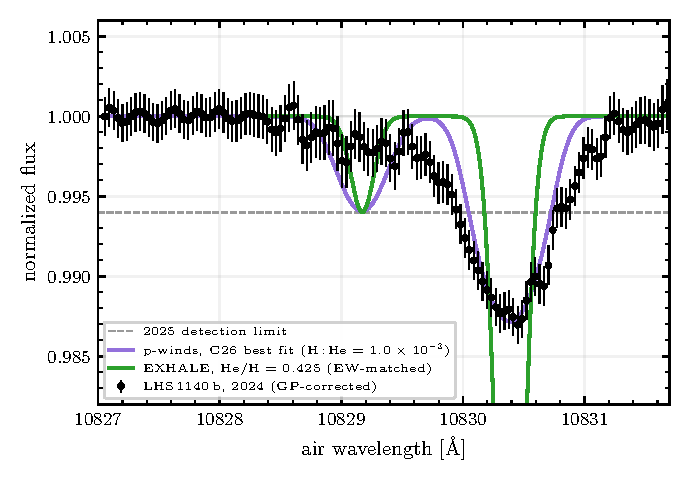
\includegraphics[width=0.60\textwidth]{figures/lhs1140b_bestfit.pdf}
\caption{The two best models over the 2024 spectrum, in the presentation of
the paper's Fig.~4: p-winds at the C26 best fit (the MCMC medians) with the
authors'
settings, and EXHALE at the equivalent-width-matched composition. Both are
shifted by the fitted $v_{\rm wind} = +2.26$\,km\,s$^{-1}$.}
\label{fig:best}
\end{figure}

Figure~\ref{fig:beststruct} shows what that EXHALE solution actually is. It
is not a fast, hot outflow: the temperature peaks at $5043$\,K near
$1.45\,R_p$ --- comparable to the isothermal value p-winds imposes --- but
then falls by adiabatic expansion to below $1000$\,K over the region that
forms the line, and the velocity reaches only $1.2$\,km\,s$^{-1}$ at
$20\,R_p$. Hydrogen is fully ionized above $\sim 3\,R_p$ while helium stays
largely neutral, and the metastable population peaks well out at
$5.4\,R_p$, $n(2\,^3S) \simeq 50$\,cm$^{-3}$. That combination --- a large,
cold, slow, metastable-rich envelope --- is precisely what produces the
right equivalent width with the wrong profile: plenty of absorbers spread
over most of the stellar disk, but almost no velocity spread to distribute
the absorption in wavelength.

\begin{figure}[!t]\centering
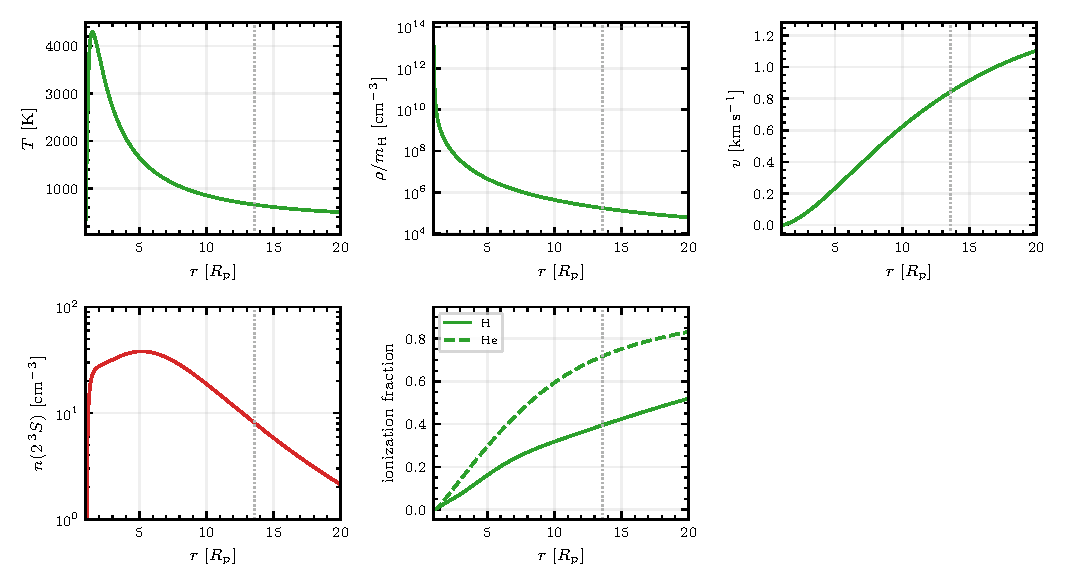
\includegraphics[width=0.92\textwidth]{figures/lhs1140b_bestfit_structure.pdf}
\caption{The EW-matched EXHALE solution ($\mathrm{He/H} = 0.55$):
temperature, density, velocity, metastable helium density, and ionization
fractions. Dotted vertical line: the stellar radius.}
\label{fig:beststruct}
\end{figure}

\section{The other proxy: five times the XUV}
\label{sec:gj699}

The first item on the list above --- more energy --- can be tested without
adding any physics, because the paper itself runs two proxy spectra. Both
stand in for LHS\,1140's unobserved XUV: GJ\,1132 (used everywhere above)
and GJ\,699, scaled to the orbit by the catalog X-ray flux ratios
$A_{1132} = 0.59$ and $A_{699} = 0.056$ following the authors' script, the
same convention adopted in Sect.~\ref{sec:sed}. Integrated over
$10$--$1300$\,\AA{} at the orbit of the planet, the GJ\,699 file carries
$169.9$\,erg\,s$^{-1}$\,cm$^{-2}$ against $33.5$ for the GJ\,1132 one: a
factor $5.1$ in XUV input.

On the EXHALE side nothing else changes. Each GJ\,699 case is the matching
GJ\,1132 input with one key replaced, \texttt{Spectrum file:}; the
luminosity keys in the file are irrelevant because \texttt{sed\_read}
overwrites them with the integral of the spectrum it reads. Each case is
started from the converged solution of the same composition on the GJ\,1132
spectrum and finished with JFNK, and all seven reach \texttt{info}~$= 0$
with $\|R\| < 10^{-3}$. One case needed a different seed:
$\mathrm{He/H} = 0.55$ stalled when started from its GJ\,1132 counterpart
and converged when restarted from the already-solved
$\mathrm{He/H} = 0.25$ GJ\,699 solution.

\subsection{Escape rate: the retrieval value, on this spectrum}

The brighter spectrum moves $\dot M$ where the composition never did:

\begin{center}
\begin{tabular}{lcc}
\toprule
 & GJ\,1132 proxy & GJ\,699 proxy \\
\midrule
$F_{\rm XUV}$ ($10$--$1300$\,\AA) [erg\,s$^{-1}$\,cm$^{-2}$]
   & $33.5$ & $169.9$ \\
$\log_{10}\dot M$ [g\,s$^{-1}$], $\mathrm{He/H} \le 1$
   & $7.75$--$7.80$ & $8.58$--$8.62$ \\
$\dot M$ [g\,s$^{-1}$] & $6\times10^{7}$ & $4.0\times10^{8}$ \\
C26 retrieval on the same proxy & $2.03\times10^{8}$
   & $4.22^{+1.14}_{-1.00}\times10^{8}$ \\
\bottomrule
\end{tabular}
\end{center}

A factor $5.1$ in XUV buys a factor $\simeq 7$ in $\dot M$ --- steeper than
linear, as expected when a larger fraction of the input goes into the wind
rather than into radiation. The result is that on this spectrum EXHALE's
escape rate agrees with the paper's retrieved value, $\log_{10}\dot M =
8.59$ against $8.63$, inside $0.02$--$0.04$\,dex and far inside the
retrieval's own $\pm 0.11$\,dex. It is also $1.4$ times the energy-limited
estimate the paper quotes for this proxy, $2.90\times10^{8}$\,g\,s$^{-1}$.
On the GJ\,1132 spectrum the same code fell a factor $3$ short of the
retrieval. Whether a solved wind and an imposed one agree on $\dot M$
therefore depends on which proxy is assumed, and the disagreement reported
in Sect.~\ref{sec:width} is not a fixed property of the code.

\subsection{Structure and line}

Seven compositions were solved on this spectrum, two of them
($\mathrm{He/H} = 0.04$ and $0.06$) placed specifically to bracket the
equivalent-width crossing:

\begin{center}
\begin{tabular}{rccccccc}
\toprule
$\mathrm{He/H}$ & $\log_{10}\dot M$ & $T_{\max}$ & $v(20R_p)$
  & $n(2\,^3S)_{\max}$ & red & FWHM & EW \\
 & [g\,s$^{-1}$] & [K] (at $r/R_p$) & [km\,s$^{-1}$]
  & [cm$^{-3}$] (at $r/R_p$) & [\%] & [\AA] & [\%\,\AA] \\
\midrule
$0.04$   & $8.58$ & $2605$ ($1.49$) & $3.61$ & $30.9$ ($5.4$) & $2.65$  & $0.270$ & $0.761$ \\
$0.06$   & $8.59$ & $2748$ ($1.48$) & $3.56$ & $47.2$ ($5.4$) & $3.83$  & $0.270$ & $1.104$ \\
$0.083$  & $8.61$ & $2896$ ($1.48$) & $3.53$ & $66.7$ ($5.5$) & $5.21$  & $0.272$ & $1.507$ \\
$0.25$   & $8.62$ & $3861$ ($1.44$) & $3.21$ & $213$  ($5.9$) & $11.98$ & $0.279$ & $3.547$ \\
$0.55$   & $8.60$ & $5079$ ($1.39$) & $2.83$ & $441$  ($6.6$) & $16.64$ & $0.288$ & $5.092$ \\
$1$      & $8.59$ & $6094$ ($1.38$) & $2.58$ & $616$  ($7.2$) & $17.28$ & $0.298$ & $5.479$ \\
$10^{3}$ & $8.43$ & $9351$ ($1.38$) & $2.07$ & $1.4\times10^{4}$ ($1.0$)
         & $105.1^{a}$ & $0.320$ & $35.87$ \\
\midrule
observed & --- & --- & --- & --- & $1.254$ & $0.841$ & $1.108 \pm 0.030$ \\
\bottomrule
\end{tabular}
\end{center}

\noindent\footnotesize $^{a}$ The three-Gaussian extractor returns the sum
of its component amplitudes, which exceeds the largest excess actually
present in the spectrum ($96.9\%$) once the line saturates into a
flat-topped trough. The entry is the fit value, kept for consistency with
every other row; it is not a depth the model reaches.\normalsize

The wind is hotter and faster than on the fainter spectrum --- at
$\mathrm{He/H} = 0.06$ it reaches $3.6$\,km\,s$^{-1}$ at $20\,R_p$ against
$1.2$ for the equivalent-width-matched GJ\,1132 solution --- and the
metastable population still peaks far out, near $5.4\,R_p$.

\subsection{The composition estimate moves by an order of magnitude}

Interpolating the equivalent width in $\log$--$\log$ across the seven
solutions and solving for the measured value gives
\begin{equation}
  \mathrm{He/H} = 0.060 \quad (0.059\text{--}0.062 \text{ on the } EW\
  1\sigma), \qquad \mathrm{H\!:\!He} = 16.6 ,
\end{equation}
with the turbulence term on, $0.060$ --- again a shift below the percent
level, so the crossing is set by the absorbing column and not by the
broadening treatment. The bracketing runs are what fix this: the two
compositions straddle the measured band directly ($EW = 0.761$ and $1.104$
against $1.108 \pm 0.030$\,\%\,\AA), so the crossing is measured rather than
extrapolated from the solar case.

This is a shift of one order of magnitude from the $\mathrm{He/H} = 0.55$
the same code gives on the GJ\,1132 proxy, and it crosses the solar value on
the way: the brighter spectrum wants a helium-\emph{poor} atmosphere,
$0.72\times$ solar, where the fainter one wanted a helium-rich one,
$6.6\times$ solar. The measurement cannot arbitrate, because the two proxies
are two guesses at the same unobserved spectrum and both reproduce the
observed equivalent width once composition is free. The conclusion to draw
is therefore about the inference, not about the planet: what the helium line
constrains is the product of composition and XUV input, and any composition
quoted from it --- the paper's $\mathrm{H\!:\!He} \lesssim 10^{-3}$ as much
as the values here --- is conditional on the assumed SED. On the present
evidence the composition inference is SED-limited.

\subsection{The width does not move}

The width is the one thing the extra energy does not fix. Across the whole
GJ\,699 scan the red-pair FWHM is $0.270$--$0.320$\,\AA{}
($0.304$--$0.377$ with the turbulence term), against the measured
$0.841$\,\AA. Measuring the deficit the way Sect.~\ref{sec:broadening} does
--- convolving with a Gaussian and asking which width reproduces the
observation --- the composition at the crossing needs
$22.1$\,km\,s$^{-1}$ FWHM of added velocity spread, against
$22.3$\,km\,s$^{-1}$ for the equivalent-width-matched GJ\,1132 solution. A
factor $5.1$ in XUV input, a factor $7$ in $\dot M$ and a factor $3$ in
outflow velocity at $20\,R_p$ change the required broadening by $1\%$.

The reason is visible in the table: the outflow velocity that grows is
radial and small compared with the missing spread, while the line-forming
region stays cold. The candidate ``more energy'' is therefore tested and
rejected as an explanation of the width. It moves $\dot M$ and it moves the
composition estimate; it does not move the profile. The remaining candidates
--- heating outside a 1D hydrodynamic energy equation, 3D velocity fields,
and an adiabatic-cooling metastable bump --- are unaffected by this test;
the last of them has since been looked for on both spectra
(Sect.~\ref{sec:bump}) and does not help either.

\begin{figure}[htbp]\centering
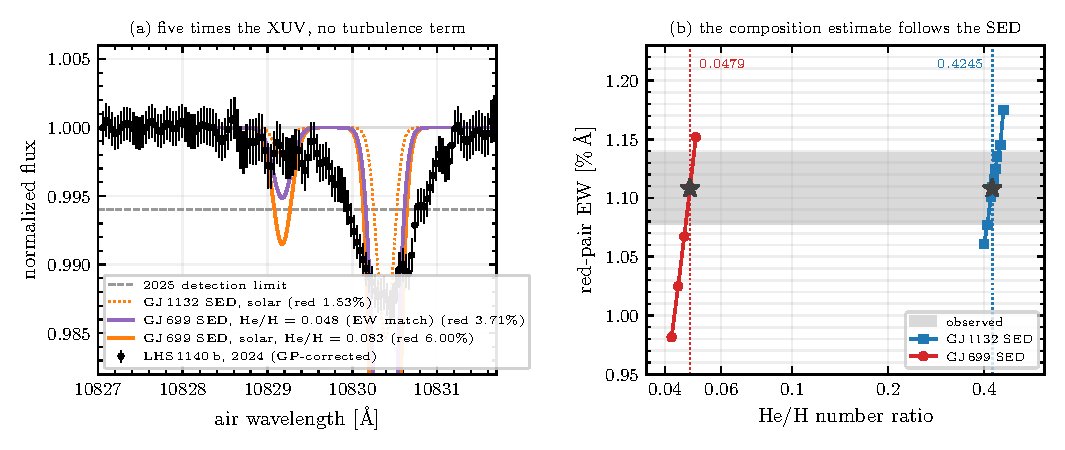
\includegraphics[width=\textwidth]{figures/lhs1140b_gj699.pdf}
\caption{The GJ\,699 proxy, five times the XUV of the GJ\,1132 proxy used
elsewhere in this memo. Left: the measurement with the EXHALE solution
nearest the equivalent-width crossing ($\mathrm{He/H} = 0.06$) and the solar
case on this spectrum, with the GJ\,1132 solar case dotted for contrast; all
curves without the turbulence term and shifted by the fitted
$v_{\rm wind} = +2.26$\,km\,s$^{-1}$. The lines are deeper and no wider.
Right: red-pair equivalent width against composition for the two spectra
with the measured band and the two crossings; the composition the line
implies moves from $0.550$ to $0.060$ when the assumed SED is changed.}
\label{fig:gj699}
\end{figure}

\section{Status against the goal}

The line is not reproduced. What stands:

\begin{itemize}
\item \textbf{Amount of absorption: matched.} $\mathrm{He/H} \simeq 0.55$,
      insensitive to the broadening treatment at the $2\%$ level.
\item \textbf{Line shape: not matched}, by a factor $3.4$ in both depth and
      width, and not fixable by composition. The missing ingredient is
      $22.3$\,km\,s$^{-1}$ FWHM of velocity spread ($\sigma =
      9.5$\,km\,s$^{-1}$), measured in Sect.~\ref{sec:broadening} and
      Fig.~\ref{fig:broadened}; supplied as one Gaussian it puts depth,
      blue depth and red/blue ratio inside the observed $1\sigma$ interval
      at once, but its physical origin is unidentified. The adiabatic
      metastable bump, which would have supplied it without a free
      parameter, is present and measured (Sect.~\ref{sec:bump}) but sits
      too slow to contribute.
\item \textbf{Escape rate: an output, not a fit, and SED-set.}
      $\dot M \simeq 6\times10^{7}$\,g\,s$^{-1}$ on the GJ\,1132 proxy, a
      third of the value the retrieval imposes, and nearly independent of
      composition. On the GJ\,699 proxy, $5.1\times$ brighter in XUV, it is
      $4.0\times10^{8}$\,g\,s$^{-1}$ --- a factor $7$ higher and within
      $0.04$\,dex of the value the paper retrieves on that same proxy
      (Sect.~\ref{sec:gj699}).
\item \textbf{Composition: SED-limited.} The equivalent-width crossing is
      $\mathrm{He/H} = 0.550$ on one proxy spectrum and $0.060$ on the
      other, helium-rich against helium-poor, with the measurement unable to
      separate them. Any composition read off this line, the paper's
      included, is conditional on the assumed XUV spectrum.
\item \textbf{One solution is not converged to tolerance.}
      $\mathrm{He/H} = 100$ stagnates at $\|R\| = 1.18\times10^{-3}$ from
      every seed tried; neighbours bracket it smoothly, so it is retained
      with the residual recorded.
\end{itemize}

\noindent That test has now been run (Sect.~\ref{sec:gj699}), and it
separated the two questions rather than answering them together: the
composition estimate moved by an order of magnitude while the width did not
move at all. The shortfall is therefore not an energy-input problem. Of the
remaining candidates the adiabatic bump has since been tested and ruled out
as a source of width for this host (Sect.~\ref{sec:bump}), which leaves the
3D and magnetic ones.

\end{document}
